\documentclass[11pt,a4paper]{article}
\usepackage[utf8]{inputenc}
\usepackage[T1]{fontenc}
\usepackage{amsthm} %numéroter les questions
\usepackage[frenchb]{babel}
\usepackage{datetime}
\usepackage{xspace} % typographie IN
\usepackage{hyperref}% hyperliens
\usepackage[all]{hypcap} %lien pointe en haut des figures
\usepackage[french]{varioref} %voir x p© y
\usepackage{fancyhdr}% en têtes
%\input cyracc.def
\usepackage[]{graphicx} %include pictures
\usepackage{pgfplots}
\usepackage[ ]{circuitikz}
\usepackage{ifthen}

\usepackage[top=1.3 in, bottom=1.3 in, left=1.3 in, right=1.3 in]{geometry} % Yeah, that's bad to play with margins
\usepackage[]{pdfpages}

\usepackage[]{attachfile}

\usepackage[many]{tcolorbox}

\newdateformat{mydate}{v1.0.0}%hack pour remplacer \THEYEAR


\newboolean{corrige}
\ifx\correction\undefined
\setboolean{corrige}{false}% pas de corrigé
\else
\setboolean{corrige}{true}%corrigé
\fi

\setboolean{corrige}{false}% pas de corrigé

\newboolean{annexes}
\setboolean{annexes}{true}%annexes
%\setboolean{annexes}{false}% pas de annexes

\definecolor{darkblue}{rgb}{0,0,0.5}

\newboolean{mos}
%\setboolean{mos}{true}%annexes
\setboolean{mos}{false}% pas de annexes

\usepackage{aeguill} %guillemets

%% fancy header & foot
\pagestyle{fancy}
%Numero du TP :
\def \labonumber {Laboratory work \no 1 }
\lhead{[ELEC-H-310] Digital Choucroute\\ \labonumber}
\rhead{\mydate\today\\ page \thepage}
\chead{\ifthenelse{\boolean{corrige}}{Corrigé}{}}
\cfoot{}
%%

\pdfinfo{
/Author (Quentin Delhaye, Ken Hasselmann, ULB -- BEAMS)
/Title (\labonumber ELEC-H-310)
/ModDate (D:\pdfdate)
}

\hypersetup{
pdftitle={\labonumber [ELEC-H-310] Digital Choucroute},
pdfauthor={Quentin Delhaye, Ken Hasselmann, ULB -- BEAMS},
pdfsubject={}
}

\theoremstyle{definition}% questions pas en italique
\newtheorem{Q}{Question}[] % numéroter les questions [section] ou non []

\newcommand{\reponse}[1]{% pour intégrer une réponse : \reponse{texte} : sera inclus si \boolean{corrige}
	\ifthenelse {\boolean{corrige}} {\paragraph{Answer~:} \color{darkblue}   #1\color{black}} {}
 }

\newcommand{\addcontentslinenono}[4]{\addtocontents{#1}{\protect\contentsline{#2}{#3}{#4}{}}}

\date{\vspace{-1.7cm}\mydate\today}
\title{\vspace{-2cm} \labonumber\\ Digital Electronics [ELEC-H-310]\\ Introduction to dsPIC\ifthenelse{\boolean{corrige}}{~\\Solution}{}}

%\author{\vspace{-1cm}}%\textsc{Yannick Allard}}

\setlength{\parskip}{0.2cm plus2mm minus1mm} %espacement entre §
\setlength{\parindent}{0pt}

\begin{document}
\pagestyle{empty}
\maketitle
% \vspace*{-1cm}
\section*{Purpose}
The purpose of this lab is to introduce a commonly used microcontroller family~: PIC from Microchip.
Few simple systems based on input/output (IO) will be realized.
In parallel, you will get familiar with C language.
Afterwards, you will learn how to realize a time-driven program.

% \section*{Prérequis}
% Il est encore conseillé de lire les sections 1 à 5 du complément «~Programmation d’une carte à microcontrôleur~».

\section*{Objectives}
At the end of this lab, you must be able to~:
\begin{itemize}
\item Write simple programs for a microcontroller.
\item Explain the idea of IOs and output current.
\item Use asynchronous elements in your code through timers.
\end{itemize}
\newpage{}


\section{Introduction}
During the six laboratories illustrating the theory, you will use a single-board microcontroller.
Besides the programming, you must understand the functioning of the various peripherals and interface them with the external world.

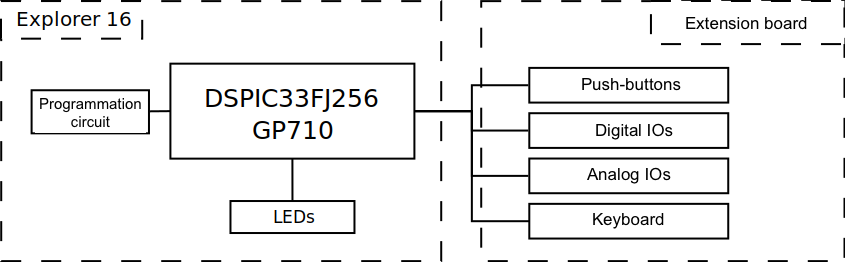
\includegraphics[width=\textwidth]{ENpic33}

This first lab will help you to get familiar with the board and use some peripherals. You will learn to interact simply with the microcontroller on the board.

The functioning of the board and the dsPic is explained in the annex «~Programmation d’une carte à microcontrôleur~».
For the first two labs, we advise you to read in particular section 4. %«~Première prise en main~».


\section{Basic programmation~: use of inputs and outputs}
Your first program will interface two sorts of IOs~: push-buttons and LEDS.
The specifications are simple~: the LED connected to the pin RA0 must switch on when a button is pushed, and switch off when this button is released.

\begin{itemize}
	\item Locate the different peripherals present on the board and named in the annex «~Programmation d’une carte à microcontrôleur~» (LEDs, push-buttons, potentiometer, analog output connected to power amplifier, etc.).
	\item With help of the annex, write the code fulfilling the specifications. Use the example code in order to:
	\begin{itemize}
		\item Locate the while(1) loop.
        This endless loop contains the tasks that must run continuously, while the code placed before and after this loop is only executed once and is mainly used to configure the peripherals and define the variables.
		\item Configure the TRIS registers of the IOs pins in order to define their role (input or output).
		\item Write the body of your program.
		\item Compile and load it on the $\mu$C board, then check its behavior.
	\end{itemize}
\end{itemize}

Later, we decide to use an high brightness LED consuming 20~mA under 3,2~V.
This LED not being present on the board, you must connect it to one of the pins of the extension board (see annex for more details).

% \par{\textbf{Rappel sur l'utilisation d'une diode.}}
% Une diode possède deux bornes~: l'anode (borne positive) et la cathode (borne négative).
% Une diode classique devant être polarisée positivement afin de laisser circuler le courant, l'anode doit être connectée à la source de tension ($\mu$C ou buffer).
% De plus, afin de limiter le courant circulant dans la diode, une résistance doit être connectée à l'anode.

\tcboxfit[height=7cm,title={Reminder on use of a diode.},
  before=\noindent]{%
  A diode has two pins~: the anode (positive pin) and the cathode (negative pin).
  Typically, a diode must be polarized positively to let the current flow, the anode must be connected to the power source ($\mu$C or buffer).
  Moreover, to limit the current passing though the diode, a resistor must be connected to the anode.

  \begin{center}
  	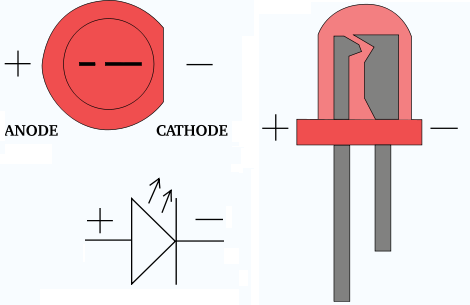
\includegraphics[width=5cm]{diagrammeLED.png}
  \end{center}

  }


\begin{itemize}
	\item Why direct connection between dsPIC and the LED does not work~?
	Link that with max output current concept.
	\reponse{
        If we connect directly the LED on an output of the board, it switches on with a very low intensity. The board is simply unable to provide enough current for the LED.
	}
	\item Explain how the use of a \textit{buffer} circuit solves this problem.
	Draw the new block diagram of your system.
	\reponse{
		The use of a buffer allows to spread the command from the microcontroller while supplying more current to the LED.
	}
\end{itemize}
We will use a buffer circuit 74ACT244 whose specifications are given in the annexes.

% \begin{itemize}
% 	\item Vérifiez que ce circuit respecte bien les normes TTL 5~V.
% 	\reponse{
% 		\begin{center}
% 			\begin{tabular}{cl}
% 			 & TTL (5~V) \\ \hline
% 			 $V_{OH}$ & 2.4 V \\
% 			 $V_{iH}$ & 2.0 V \\
% 			 $V_{iL}$ & 0.8 V \\
% 			 $V_{OL}$ & 0.5 V \\
% 			\end{tabular}
% 		\end{center}
% 		~\newline{}

% 		Dans notre montage, l'entrée à l'état haut est à 3.3~V et la basse à 0~V (imposés par la carte).
% 		Étant donné que ces valeurs sont resectivement plus haute que $V_{iH}$ et plus basse que $V_{iL}$ en TTL 5~V, la norme est respectée.
% 	}
% 	\item Réalisez un montage sur protoboard permettant d’allumer la LED.
% 	N’oubliez pas de dimensionner la résistance de limitation du courant dans la diode.
% 	Alimentez le buffer en 0~V/5~V
% 	\item Modifiez votre programme pour qu’une pression sur le bouton allume désormais la LED ultra-brillante externe au lieu de celles présentes sur la carte.
% \end{itemize}



\section{Use of the timer}
You are asked to make the LEDs blink at a given frequency.
To do so, you will need a timer.
This peripheral has a 16 bits register incremented at each clock cycle.
When the value of this register reaches the value in the period register (PR1 for timer 1, PR2 for timer 2, etc.), the counter goes back to 0 and starts incrementing again.
At the same time, a specific bit named flag rises (goes to '1') to warn of overflow (cf. guide).
As a first step, you will write a program allowing to make the LED blink at a frequency of 10~kHz.

\begin{itemize}
	\item What must be the value in the PR register of the timer in order to cause an overflow at the good frequency~?
    What is the largest period of the timer~? As a reminder, the processor instruction execution rate is 40~MHz.
	\reponse{
		If we want the LED to blink at a frequency of 10~kHz, the state of its pin must change with rate of 20~kHz. For the timer, this corresponds to a period of 2000 instructions. The maximum period of this timer (on 16 bits) is $\frac{2^{16}-1}{40\cdot10^6} = 1638 \mu s$. Using a \textit{prescale} of 256, this periode can go up to $0,419 s$ .
	}
	\item Check that the call of the function \texttt{clav2LCD} is commented out.
	\item Add the configuration and launching of the timer of your choice in your program.
	\item In the main loop of your program~:
	\begin{itemize}
		\item Check by polling if the timer has overflowed (ie. If the bit TxIF has risen to '1').
		\item Write a function that toggles pin RC1 at overflow frequency. This function must not be blocking~: the high brightness LED must switch on at any time if the button is pressed.
		\item Do not forget to reset (set to '0') the TxIF bit in your program.
	\end{itemize}
	\item Check the frequency with the oscilloscope.
	\item Modify the function to set the period to 500~ms and program the blinking of the LEDs.
	\reponse{
		As the state change period is about 250~ms, a 16 bit timer can still be used if coupled to a 256 \textif{prescaler}.
	}
\end{itemize}

\end{document}
